\documentclass[11pt, oneside]{article}
\usepackage{geometry} % see geometry.pdf on how to lay out the page. There's lots.
\geometry{letterpaper} % or letter or a5paper or ... etc
% \geometry{landscape} % rotated page geometry
\usepackage{graphicx}

\usepackage{amssymb}
\usepackage{amsmath}
\usepackage{inconsolata}
% See the ``Article customise'' template for come common customisations

\title{Introduction to Programming with HERB}
\author{HERB Lab}
\date{2013-09-06} % delete this line to display the current date

%%% BEGIN DOCUMENT
\begin{document}

\maketitle


\section{Simulation}

\subsection{Herbpy Console}
\begin{figure}[htbp]
   \centering
   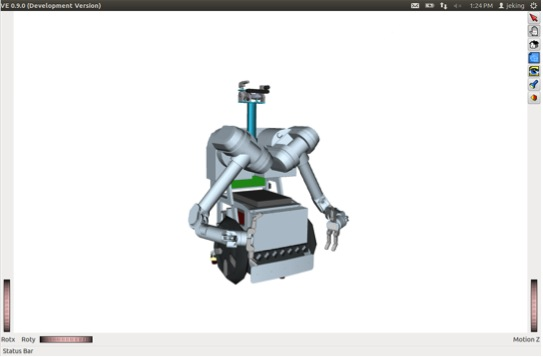
\includegraphics[width=0.8\textwidth]{figs/viewer.jpg} % requires the graphicx package
   \caption{The herbpy viewer}
   \label{fig:viewer}
\end{figure}
The easiest way to work with HERB in simulation is via the herbpy console.  To start up a herbpy console in simulation mode type the following from a command line:
\begin{figure}[h]
\centering

\includegraphics[width=0.6\textwidth]{figs/herbpystart.jpg}
\end{figure}
Here the parameter \texttt{sim} indicates you would like to start in simulation mode. The parameter \texttt{viewer} indicates that a viewer should be attached to the instance.  Figure~\ref{fig:viewer} shows an example of the viewer.  

An additional parameter that is useful is \texttt{debug}.  This will set the logging level to DEBUG.  By default, the log level is set to INFO.

Starting the herbpy console will drop into an ipython prompt.  Two useful objects have been initialized: \texttt{robot} and \texttt{env}. 

\subsubsection{\texttt{robot}}
The \texttt{robot} objects is a pointer to the model of the robot, in this case HERB.  Many operations on the robot are available.  For example, the following will give the current value of all 24 DOF values for the robot:
\begin{figure}[h]
\centering
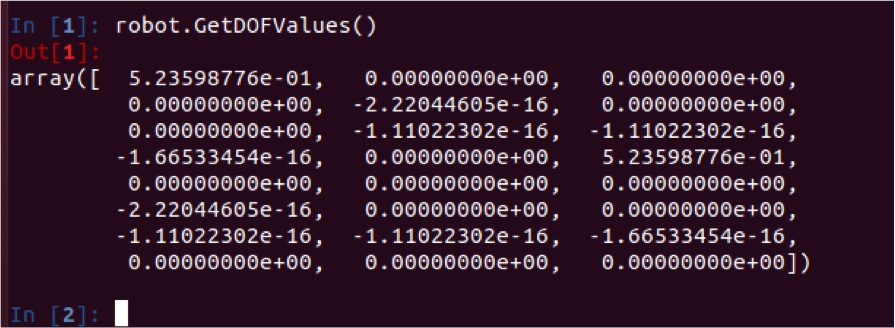
\includegraphics[width=0.8\textwidth]{figs/getdofvalues.jpg}
\end{figure}

Pointers exist for each arm of the robot via calls to \texttt{robot.left\_arm} and \texttt{robot.right\_arm}.  The following command gets DOF values for only the right arm:
\begin{figure}[h]
\centering
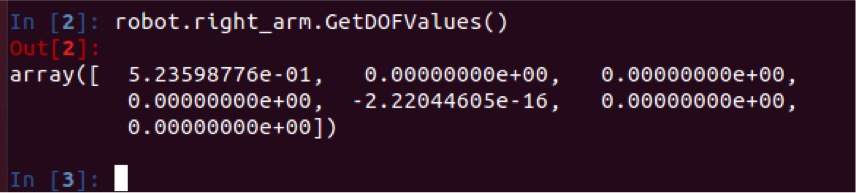
\includegraphics[width=0.8\textwidth]{figs/getrightdofvalues.jpg}
\end{figure}

Several planners exists for planning motions for the arms.  A common one, developed in this lab, is the CHOMP planner.  Prior to using the CHOMP planner, the distance field must be initialized.  The following command performs this initialization:
\begin{figure}[h]
\centering
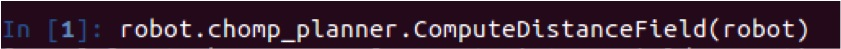
\includegraphics[width=0.8\textwidth]{figs/chompinitialize.jpg}
\end{figure}



\section{Real Life}

\section{Python Scripting}

\end{document}